\documentclass[a4paper,twoside]{article}

\usepackage{pslatex}
\usepackage{hyperref}
\usepackage[hyphenbreaks]{breakurl}
\usepackage{breakurl}

\usepackage{epsfig}
\usepackage{array}
\usepackage{dcolumn}

\usepackage{SCITEPRESS}
\usepackage{multicol}

\usepackage{apalike}
\bibliographystyle{apalike}

\usepackage[small]{caption}

\begin{document}

\title{INSTRUMENTAL ENVIRONMENT OF MULTI-PROTOCOL CLOUD-ORIENTED VEHICULAR MESH NETWORK}

\author{\authorname{Glazunov Vadim, Kurochkin Leonid,  Kurochkin Mihail and Popov Sergey} \affiliation{Telematics department, Saint-Petersburg State Polytechnic University, Polytechnicheskaya st. 29, Saint-Petersburg, 195251, Russia} \email{\{neweagle, kurochkinl, kurochkin.m\}@gmail.com, popov.sergey@rtc.spbstu.ru}
}

\keywords{Digital communication protocol, MESH network, traffic network, interface, route protocol, cloud service, interface network capacity, network traffic.}

\abstract{The article deals with issues of message transfer adequacy in the cloud-oriented vehicular MESH network, specification of message delivery time with different traffic network configuration, vehicular traffic density, network traffic density.}

\onecolumn \maketitle \normalsize \vfill

\section{INTRODUCTION}

Nowadays a greater attention has been paid to researches of issues of cloud-oriented vehicular MESH network construction. Constant enhancement of communications transmission media, network hardware, methods of inter-network interaction and access to cloud services allow to set new tasks of providing information services to information network users. Special interest is paid to issues of quality increase of message exchange between transport networks users in the process of movement in unstable connection areas~\cite{Zaborovsky}.

Messages exchange between a vehicle and a cloud is done through a communication channel with the cloud detached to the vehicle organized by means of automotive telematics devices, or user's personal devices such as smart phones, laptops and public cellular networks in communication mode. Service quality in the cloud-oriented environment is determined by third-party equipment reliability and cellular networks coverage quality~\cite{6083854}.

Organization of a mobile self-organized local vehicular network with exit points to the cloud environment has been considered as a perspective direction of information network development in unstable coverage areas. In such model message exchange between the vehicle and the cloud can be fulfilled through several alternative paths, and a vehicular aggregate on the route can be regarded as a mobile local network with altering topology and composition with a variable number of communication transmission points with the cloud network. MESH network is a perspective technology of communication transmission between vehicles and the cloud environment. Most of the authors who work in this direction study models of networks with stationery signal relays.

The paper~\cite{6466777} deals with issues of the cloud-oriented MESH environment construction with a regular structure of stationery network points. It proves a necessity of development of a new multi-address communication protocol in the MESH environment based on data of vehicles and stationary points location. Authors consider issues of structure of the MESH-environment information control system that is oriented at vehicles.

The paper~\cite{6008765} offers a structure of automotive information system, conception of access sceneries to cloud environment and customer sceneries of interaction with the cloud.

The paper~\cite{6215525} is dedicated to the description of technology environment of wireless vehicular networks traffic modeling with application of the NS-3 simulator libraries.

The paper~\cite{6133884} offers the network with a one-step signal relay through a vehicle equipped with LTE transmitter.

The paper~\cite{5719268} describes algorithms of forming and simulating of dynamic VANET clusters for access to global services.

\section{INTERACTION OF NETWORK OBJECTS WITH THE CLOUD ENVIRONMENT}

Most of the researchers pay no attention to the situation of continuous communication lack with a stationary transmitter when immediate communication transfer is impossible. Meantime if each vehicle is regarded as a mobile transmitter it is possible to provide message transfer with the cloud through communication transfer via them. The choice of communication transfer point to the cloud environment appears if numerous access points to the cloud exist.

\begin{figure*}[!ht]
  \vspace{-0.2cm}
  \centering{
    \epsfig{file = fig1big.eps, width = 15.8cm}
  \caption{Scheme of interaction of single-rank heterogeneous network objects with the cloud environment.}
  \label{fig:Fig1}}
  \vspace{-0.1cm}
\end{figure*}

Present day classical algorithms of MESH networks route search are used to build access routes to the cloud environment. They offer the search of single route to a unique pre-known user. In the case of the cloud-oriented service it is required to make a choice of the most perspective point from several alternatives. It is necessary to find an available point with the cloud access and to evaluate perspective of communication transfer and receipt through them~\cite{gramaglia:seamless}.

Figure~\ref{fig:Fig1} presents the chart of interaction of single-rank heterogeneous network objects with the cloud environment.

Communication with the cloud can be implemented in two ways: by the vehicle with communication equipment and by the stationery point. The vehicle situated out of communication area can access the cloud through a vehicle transmitter chain. The network provides a bidirectional message transfer --- from the vehicle to the cloud and inversely.

The most important task of such network building is the alternative choice of communication protocol usage for increasing message transfer adequacy. Estimation of message time delivery to cloud services and the MESH network users depends on vehicle traffic intensity, communication network download traffic, interface availability and its composition in vehicles.

This paper studies the problem of message transfer adequacy increase between the cloud environment and the MESH (802.11s) network.

A set of interfaces that allows being a user of LTE and MESH networks concurrently or MESH only (communication between vehicles only) is installed on vehicles (network points). The double-interface point (LTE, 802.11s) serves as a gateway providing communication between the MESH network and the cloud environment through LTE.

Dependencies of message transfer adequacy, design and actual communication speed relations, mean lag of message delivery during interaction of the point with the cloud environment depending on used route protocol and intensity of communication streams are determined in the frame of the research.

Features of the communication network in question given in figure~\ref{fig:Fig2} are following:

\begin{itemize}
\item[$-$] lack of a stable communication channel between the vehicle and the cloud;
\item[$-$] necessity of message transfer via MESH to the point that has an access to the cloud environment (LTE).
\end{itemize}

\section{NS-3 NETWORK CORE MODULES AND EXTERNAL MODELS}

Basic research method is a simulation modeling of the network function in NS-3 environment (discrete-event simulator of telecommunication systems~\cite{Nsnam.org}.

NS-3 simulator is a free software licensed under the GPL license. It is targeted for research and educational use. NS-3 source codes are opened for research, modification and usage and available at the project's site. C++ and Python are used as an embedded language for model description.

Models of wire and wireless network that allow simulating mixed networks with various complexity topologies are developed in the NS-3. Special interest in this paper is given to the MESH networks realization on the base of 802.11s stack protocol.

Intelligent Driver Model (IDM) was used to build a vehicular network and model highway mobility~\cite{citeulike:10001487}.

IDM describes movement of the vehicle on the highway network taking into account the vehicle location on traffic lanes, vehicle's overall dimensions, distance between vehicles, vehicle's behavior at the lane change, lane traffic direction, average speed and acceleration in the given lane, traffic lights signals, traffic allocation on cross-roads~\cite{5678993}.

Simulation was carried out in the NS-3 simulator (v.3.16). The IDM model realization redesign connected with adaptation of its data structures to the latest version of the NS-3 (v.3.16) was fulfilled to coordinate the NS-3 and IDM versions.

A model of mobile point with a set of network interfaces was developed to perform experiments.

To synthesize a multi-protocol point a new class was added to the IDM model. It enlarged a list of point available interfaces with a following set: 802.11abg, 802.11s, LTE. Primarily the interface set was limited with a 802.11s interface.
In the process of simulation the movement of the multi-protocol mobile point is made with setting the parameters of mobile traffic scheme. Change of vehicle coordinates leads to change of multi-protocol mobile point coordinates. The vehicle is moved discretely in the interval of 0.1 sec during all the period of modeling.

Method of variable parameters initialization is developed to conduct the research. It includes an "access to cloud" point feature, a route protocol, a communication speed, number of points in the traffic, number of points with simultaneous transmission, size of transmitted packages, vehicular communication protocol. Measurable parameters are time of package sending, time of package delivery, number of lost packages, package size, IP addresses of sources and message recipients.

\section{IMPLEMENTATION}

\subsection{Creation of Multi-Protocol Point}

The NS-3 simulator v. 3.16 does not give a ready solution for creation of a multi-protocol point that serves as a gateway between 802.11s and LTE networks (figure~\ref{fig:Fig2}). Building of simulation model of mobile communication network required realization of a multi-protocol point model (figure~\ref{fig:Fig3}) functioned as message routing between 802.11s and LTE communication networks. Realization of a multi-protocol point is made on the base of a "spot-to-spot" virtual point enabled intermediate interaction between 802.11s and LTE interfaces.

To implement a model with the multi-protocol point that provides interaction of LTE and MESH networks it is required to carry out following actions:

\begin{enumerate}
\item to create points with a 802.11s interface (NodeContainer class);

\item to program movement model of LTE points (it is important to make this before installation of UE and eNB interfaces)~\cite{LTE};

\item to install LTE base station points (eNB, InstallEnbDevice method, LteHelper class);

\item to install LTE clients points (UE, InstallUeDevice method, LteHelper class);

\item to create a "spot-to-spot" virtual point that serves as an intermediate link to connect LTE and MESH interface;

\item to add LTE interface in MESH point (Add method NodeContainer class);

\item to create a gateway to connect LTE with extranet (GetPgwNode method EpcHelper class);

\item to assign IP-addresses to network points including virtual point (Assign method Ipv4InterfaceContainer class);

\item to add a route from a chosen point to LTE network via intermediate multi-interface point with MESH and LTE (AddNetworkRouteTo method Ipv4StaticRouting class);

\item to set route on default on LTE interfaces (through a gateway in this network, a gateway address is got by GetUeDefaultGatewayAddress method EpcHelper class and set by SetDefaultRoute method Ipv4StaticRouting class).
\end{enumerate}

\begin{figure}[!h]
  \vspace{-0.2cm}
  \centering{
    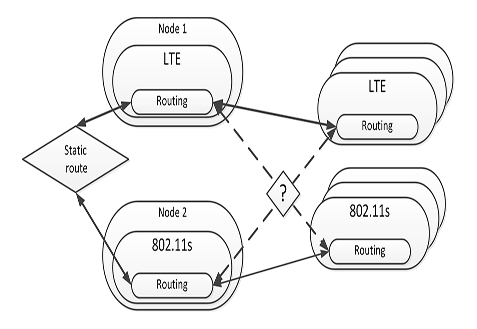
\epsfig{file = fig2.eps, width = 7.5cm}
  \caption{Basic implementation of gateway 802.11s-LTE.}
  \label{fig:Fig2}}
  \vspace{-0.1cm}
\end{figure}


\begin{figure}[!ht]
  \vspace{-0.2cm}
  \centering{
    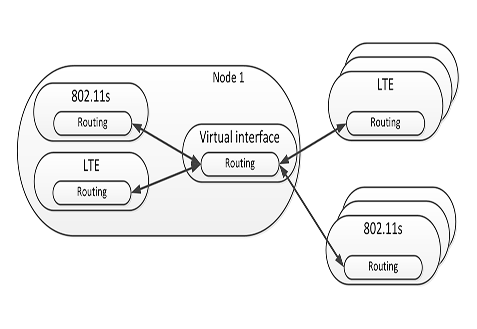
\epsfig{file = fig3.eps, width = 7.5cm}
  \caption{Implementation of the multi-protocol point.}
  \label{fig:Fig3}}
  \vspace{-0.1cm}
\end{figure}

The chart given at figure~\ref{fig:Fig3} allows message delivering from any MESH network point to the cloud.

\subsection{Special Features of the Model Program Implementation}

Modules NS-3 used in the process of model implementation:
\begin{itemize}
\item[$-$] 802.11s interface model~\cite{Andreev}. Implementation enables by default to use the HWMP route protocol in proactive and reactive modes, in addition to that route protocols for wireless MESH networks will be used: OLSR, AODV, DSDV.

\item[$-$] implementation of route protocol models in wireless networks HWMP, OLSR, AODV, DSDV~\cite{Narra:2011:DDV:2151054.2151132};

\item[$-$] FlowMonitor is a module of network traffic statistics collecting and processing that provides various methods of modeling network devices and communication channels specification collecting;

\item[$-$] WireShark is an analyzer of computer network traffic that gives broad opportunities to filter and sort traffic data of various network protocols;

\item[$-$] PyViz is a module of model visualization that allows to show topology of a modeling network, data traffic, specifications of interfaces and channels and their alteration during simulation process as well;
\end{itemize}

\subsection{NS-3-highway-mobility is a model of vehicular traffic.}
The given chart (fig.4) of modules interaction allows combining various route protocol, network interfaces, and models of network point mobility within the NS-3 simulator. 

Parameters of simulation are sent to NetworkNodes class where choice and route protocol setting is implemented, several network interfaces are created, and speed of communication, number of transmitting points and type of network traffic are set up. Simulation is resulted in a set of xml-files generated by the FlowMonitor module.

One network points is equipped with LTE interface (it sends data to the cloud environment), data from other network users are sent to it. 

Valid values of simulation parameters prescribed by such limits allows researching the most dynamic periods of the MESH network existence (short time of the network life, wide range of network traffic intensity, high intensity of route relocation).

\begin{table}[!ht]
\caption{Experiments initial data.}\label{tab:initialdata} \centering
\begin{tabular}{ p{3.28cm} | p{3.28cm}}
  \hline
  Parameter & Value \\
  \hline  \hline
  Network & 802.11s, LTE \\
  \hline
  Quantity of network points & 4--16 \\
  \hline
  Highway fragment & 200m x 200m with two-way traffic \\
  \hline
  Communication intensity from the point to the cloud & 8--2048 Kbit/s \\
  \hline
  Maximal speed of the point & 50 km/h \\
  \hline
  Message size & 1024 bytes \\
  \hline
  Route protocols & HWMP, OLSR, AODV, DSDV \\
  \hline
  Traffic type & TCP, UDP \\
  \hline
\end{tabular}
\end{table}

\begin{figure*}[!ht]
  \vspace{-0.2cm}
  \centering{
  \epsfig{file = fig4big.eps, width = 15.8cm}
  \caption{Presents the environment structure of heterogeneous network model.}
  \label{fig:Fig4}}
  \vspace{-0.1cm}
\end{figure*}

\section{ANALYSIS OF RESULTS}

\subsection{Estimation of Design and Actual Communication Speed Relations}

Research of actual communication speed was carried out for different routing protocol and short time of network life. Routing protocols in wireless MESH networks OLSR, DSDV, AODV and the HWMP protocol developed specially for 802.11s were studied for comparison. The UPD traffic sent with speeds of 8, 32, 64, 128, 512, 1024, 2048 Kbit/s was used in the experiment. Relation of actual data transfer rate to network communication speed is given in figure~\ref{fig:Fig5} and figure~\ref{fig:Fig6} shows relation of design data transfer rate to actual one.

\begin{figure}[!ht]
  \vspace{-0.2cm}
  \centering{
  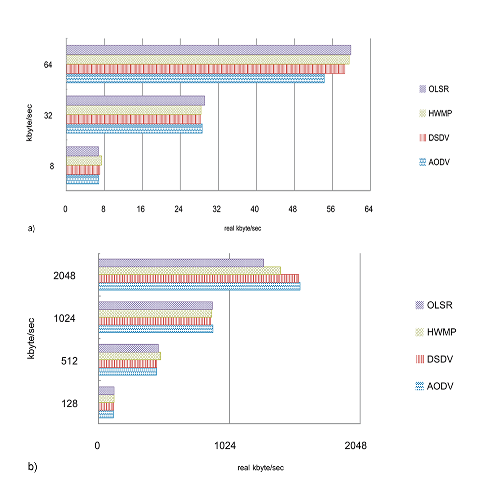
\epsfig{file = fig5.eps, width = 7.5cm}
  \caption{Actual data transfer rate for different routing protocols: for 8-64 (a), 128-2048 (b) Kbit/s transfer speed.}
  \label{fig:Fig5}}
  \vspace{-0.1cm}
\end{figure}

Actual data transfer rate in the mobile network is lower than design one due to generation of service traffic required by routing protocols to support of actual data of network topology state. Interval of actual speed decrease makes up from 5 to 37\%. Substantial decrease of actual communication speed (up to 35\%) is observed at speeds over 1024 Kbit/s required for transfer media data. AODV and DSDV protocol shows best results with high intensity streams. HWMP protocol demonstrates the highest speed of short messages transfer with low intensity.
 
\begin{figure}[!ht]
  \vspace{-0.2cm}
  \centering{
  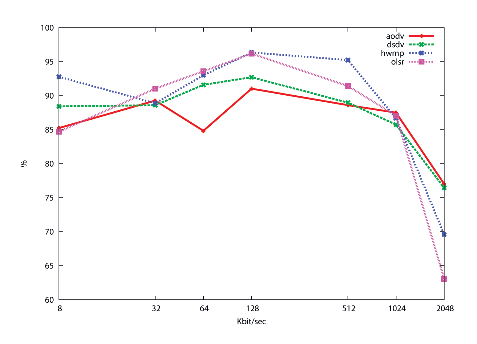
\epsfig{file = fig6.eps, width = 7.5cm}
  \caption{Relation of design and actual data transfer rates.}
  \label{fig:Fig6}}
  \vspace{-0.1cm}
\end{figure}

\subsection{Estimation of Delivered Messages Number}

Number of delivered messages was defined for the most difficult modes of the network existence when the time of the vehicle staying in the network is less than 1 second. Constant work of routing protocol and a significant percentage of lost messages are typical for them. Following factors were taken into account in a simulation process with fixed number of mobile transmitters of a mobile point~-~16.

\begin{figure}[!ht]
  \vspace{-0.2cm}
  \centering{
  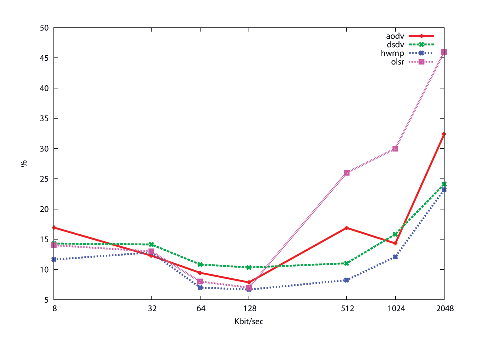
\epsfig{file = fig7.eps, width = 7.5cm}
  \caption{Percentage of lost messages.}
  \label{fig:Fig7}}
  \vspace{-0.1cm}
\end{figure}

\subsection{Estimation of Average Time of Message Transfer through the Route}

Average time of message transfer from the user to the mobile transmitter that has a communication channel with the cloud for different number of points (8 and 16), for the HWMP routing protocol.

Following parameter points were given during simulation process with 512 Kbit/s average data transfer rate and TCP traffic.

At this parameters average time of message delivery from the user to the cloud environment made 70,41 ms for 8 points and 4.04 ms for 16 points. Reduction of message delivery time for 16 points is connected with the increase of communication routes number.

\section{CONCLUSION AND FUTURE WORK}

The research has led to the following results:

statement of urgent problem of studying behavior of mobile wireless communication network on the base of 802.11s, LTE directed at usage of the cloud environment services;

development of wireless communication model based on the IDM that differs from analogues with multi-protocol points provided interaction of 802.11s, LTE networks and the cloud environment;

selection of the set of parameters and parameter domain: routing protocol, communication traffic intensity, number of network points, etc. that allows studying periods of the greatest alteration of the structure and state of mobile wireless communication network;

estimation of security level of data transfer, actual speed of data transfer supported by the network and average time of message exchange of the network point with the cloud environment.

It is planned to make a detailed research of temporal features, to analyze possibility of building optimal routes of message re-sending between the network point and the cloud environment, to develop a universal routing protocol for a multi-protocol cloud-oriented vehicular MESH network based on the current research.

\bibliography{implementation}{}

\end{document}
